\chapter{Knapsack Problem 0/1 - Il Problema dello Zaino 0/1}
Questione da risolvere: trovare il subset di oggetti di massimo valore complessivo
che non superi la capacità C.
\paragraph*{Oggetti} Ad ogni oggetto viene associato un peso e un valore, quindi il problema
consiste nel inserire nello zaino il massimo valore possibile senza superare il peso massimo.
\section{Istanza del problema}
Insieme di n oggetti $\{1,2,\dots,i,\dots,n\}$:
\begin{itemize}
    \item C \ra Capacità dello zaino
    \item $v_n$ \ra Valore dell'oggetto n
    \item $w_n$ \ra peso/ingombro dell'oggetto n
\end{itemize}
\paragraph*{Esempio}
\begin{center}
    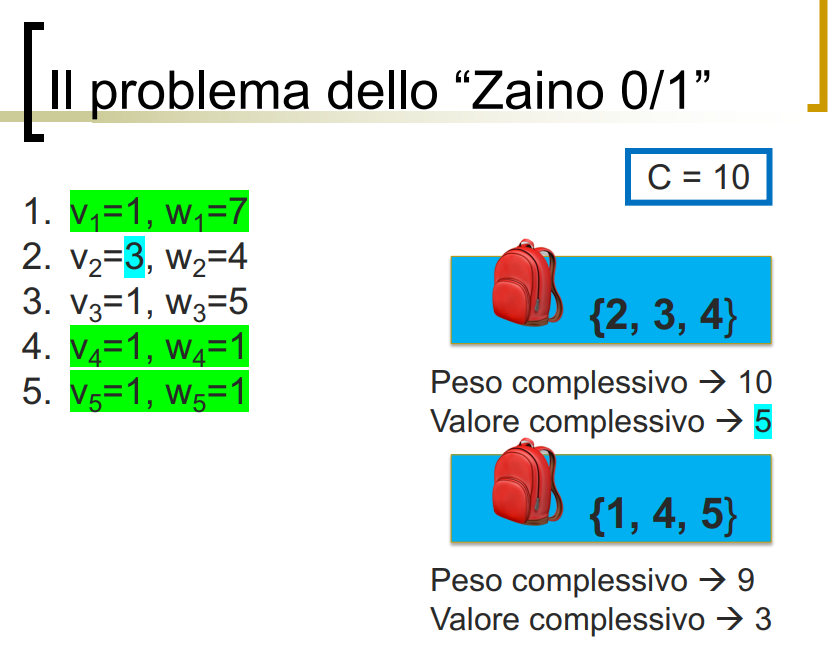
\includegraphics[width=100mm, scale=0.5]{chapters_ulerich/img/knapsack_example.png}
\end{center}
\section{Definizione formale}
Dato un insieme $X=\{1,2,\dots,i,\dots,n\}$ di n oggetti, un intero C e due funzioni:
\begin{itemize}
    \item $V:X \rt N$ tale che $V(i) = v_i$ è il valore dell'oggetto i
    \item $W:X \rt N$ tale che $W(i)=w_i$ è il peso dell'oggetto i
\end{itemize}
si vuole trovare un sottoinsieme $S=\{i_1,i_2,\dots, i_k\}$ di X tale per cui:
\begin{align*}
    W_S=&\sum^k_{j=1}w(i_j) \leq C\\
    V_S=&\sum^k_{j=1}v(i_j)
\end{align*}
Dove $V_S$ è il massimo tra tutti i valori dei possibili sottoinsiemi di X che sono "compatibili" con lo zaino.\\
Si tratta dunque di un problema di ottimizzazione di massimo, dove:
\begin{itemize}
    \item (n,C) \ra dimensione del problema
    \item Soluzioni possibili \ra tutti i sottoinsiemi $S'$ di X il cui peso totale $W_{S'}$ è al più la capacità C
    dello zaino
    \item Funzione obiettivo \ra valore totale $V_{S'}$ della soluzione possibile $S'$.
    \item Valore totale di S \ra valore ottimo
    \item S \ra Soluzione ottimale
\end{itemize}
\subsection{Soluzione del problema DP}
\begin{enumerate}
    \item Calcolo del valore ottimo (valore totale di S)
    \item Ricostruzione di una soluzione ottimale (un insieme S)
\end{enumerate}
\section{Sottostruttura Ottima}
Consideriamo l'esempio di inizio capitolo:
\begin{center}
    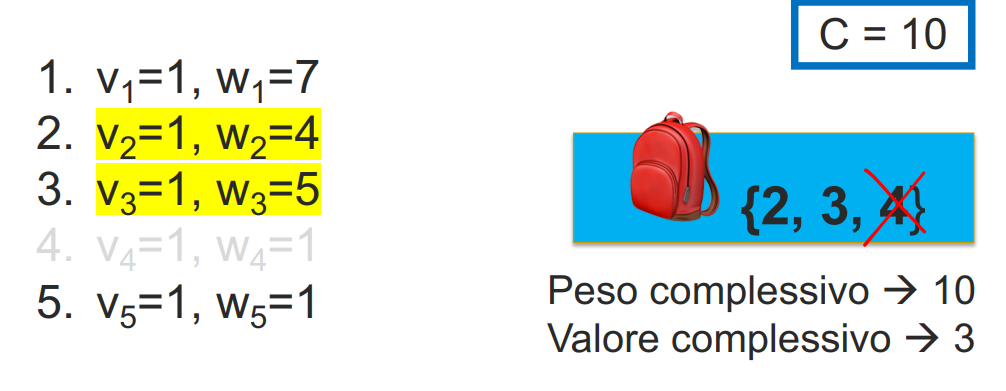
\includegraphics[width=80mm, scale=0.5]{chapters_ulerich/img/knapsack_ricerca_sott_ott.png}
\end{center}
$\{2,3\}$ è una soluzione ottimale di $X \setminus \{4\}$? \textcolor{red}{NO}.\\
$\{2,3, 5\}$ è una soluzione ottimale di $X \setminus \{4\}$!\\
\subsection{Diamo un ordine agli oggetti}
Diamo un ordine agli oggetti all'interno di X, cioè:\\
1 viene prime di 2 che viene prima di 3, etc. che viene prima dell'ultimo oggetto n.\\
\paragraph*{Data una soluzione ottima S si può verificare}
\begin{itemize}
    \item \textbf{CASO 1}: l'oggetto n appartiene a S
    \item \textbf{CASO 2}: l'oggetto n NON appartiene a S
\end{itemize}
\subsection*{CASO 1 $C \geq w_n$ e l'oggetto n appartiene a S}
\paragraph*{NB:} $S' = S \setminus \{n\}$ non è necessariamente la soluzione ottimale dell'istanza per
$X \setminus \{n\}$ e capacità C.\\
Infatti, se esiste $i \in X \setminus \{n\} \text{ t.c } i \notin S' \text{ e } w_i \leq C - W_{S'} 
\implies S' \cup \{i\}$ ha valore totale maggiore di quello di $S'$.\\
Tornando a noi, CASO 1 implica che $\implies S' = S \setminus \{n\}$ è soluzione ottimale per 
l'istanza data da:
\begin{itemize}
    \item insieme di oggetti $X \setminus \{n\} = \{1,2,\dots,n-1\}$
    \item Zaino di capacità $C'$ pari a $C-w_n$
\end{itemize} 
\begin{center}
    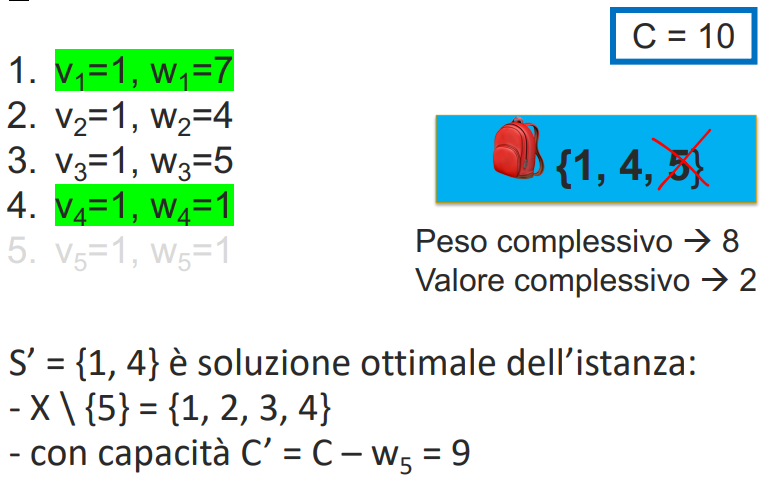
\includegraphics[width=90mm,scale=0.5]{chapters_ulerich/img/knapsack_n_in_S.png}
\end{center}
\subsection*{PROOF} 
\begin{enumerate}
    \item $S'$ è compatibile con la capacità $C-w_n$\\
    $W_S \leq C \implies W_S - w_n \leq C - w_n \implies W_{S'} \leq C- w_n$
    \item $S'$ ha valore totale $V_{S'}$ massimo\\
    Se esiste $S''$ tale che $V_{S''} > V_{S'}$ e $W_{S''} \leq C-w_n$\\
    $\implies S'' \cup \{n\}$ è soluzione ottimale per l'istanza X e C di valore totale
    maggiore di $V_S$ (contro l'ipotesi)
\end{enumerate}
\subsection*{CASO 2 - L'oggetto n NON appartiene a S}
$\implies$ S è soluzione ottimale per l'istanza data da:
\begin{itemize}
    \item insieme di oggetti $X \setminus \{n\} = \{1,2,\dots,n-1\}$
    \item Zaino di capacità pari a C
\end{itemize}
Non avendo aggiunto l'oggetto allo zaino la capacità totale rimane invariata.
\begin{center}
    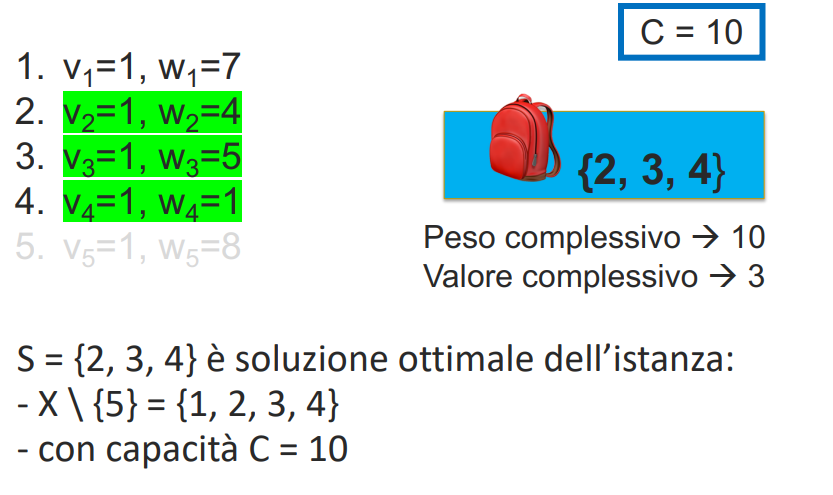
\includegraphics[width=90mm,scale=0.5]{chapters_ulerich/img/knapsack_n_notin_S.png}
\end{center}
\subsection*{PROOF}
Se esiste $S'$ che è soluzione ottimale per $X \setminus \{n\}$ e capacità C e con
valore $V_{S'} > V_{S'}$ allora $S'$ sarà soluzione ottimale per X e capacità C (contro
l'ipotesi).
\subsection{Sottostruttura ottima}
Dato un insieme $X=\{1,2,\dots,n\}$ di n oggetti, uno zaino di capacità C e una soluzione
ottimale S:\\
$C \geq w_n, \, n \in S \implies S' = S \setminus\{n\}$ è soluzione ottimale per:
\begin{itemize}
    \item insieme di oggetti $\{1,2,\dots, n-1\}$
    \item capacità $C-w_n$
\end{itemize}
\begin{mdframed}[backgroundcolor=lightgray]
    Problema $(n-1, C-w_n)$    
\end{mdframed}
\textbf{$S = S' \cup \{n\}$} con $S'$ soluzione ottimale per le condizioni viste prima del box.
$n \notin S \implies S$ è soluzione ottimale per:
\begin{itemize}
    \item insieme di oggetti $\{1,2,\dots,n-1\}$
    \item capacità C
\end{itemize}
\begin{mdframed}
    Problema $(n-1,C)$
\end{mdframed}
$S = S''$ con $S''$ soluzione ottimale per le condizioni viste prima del box.
\subsection{Passo ricorsivo per (n,C)}
Dato un insieme $X=\{1,2,\dots,n\}$ di n oggetti e uno zaino id capacità C, la soluzione
ottimale $S_{n,C}$ è:\\
\textbf{Se $C \geq w_n$ allora}
\begin{itemize}
    \item $S_{n,C} = max_V\{S' \cup \{n\},S''\}$
\end{itemize}
\textbf{altrimenti}
\begin{itemize}
    \item $S_{n,C} = S''$
\end{itemize}
$S'$ soluzione ottimale per il problema $(n-1, C-w_n) \rt S_{n-1,C-w_n}$\\
$S''$ soluzione ottimale per il problema $(n-1,C) \rt S_{n-1,C}$
Sostituisco nelle equazioni $S'$ e $S''$:
\textbf{Se $C \geq w_n$ allora}
\begin{itemize}
    \item $S_{n,C} = max_V\{S_{n-1, C-w_n} \cup \{n\},S_{n-1, C}\}$
\end{itemize}
\textbf{altrimenti}
\begin{itemize}
    \item $S_{n,C} = S_{n-1,C}$
\end{itemize}
\subsection{Definizione dei sottoproblemi}
\paragraph*{Sottoproblema di dimensione (i,c)}
Riempire uno zaino di capacità c con oggetti dall'insieme $\{1,2,\dots,i\} \rt S_{i,c}$\\
$i \in \{1,2,\dots,n\}$\\
$c \in \{0,1,\dots,C\}$
\paragraph*{Numero di sottoproblemi:}$(n+1)(C+1)$
\begin{mdframed}[backgroundcolor=yellow]
    $i=n,\, c=C$ \ra problema principale
\end{mdframed}
\section{Equazioni di ricorrenza}
\paragraph*{CASI BASE} \ra Tutti i sottoproblemi di dimensione $(i,c)$ tale per cui i = 0, oppure
C = 0.
\[S_{i,C} = \emptyset\]
\paragraph*{PASSO RICORSIVO} \ra Tutti i sottoproblemi di dimensione $(i,c)$ tale per cui
$i>0$ e $c>0$.\\
\textbf{Se $C \geq w_n$ allora}
\begin{itemize}
    \item $S_{n,C} = max_V\{S_{n-1, C-w_n} \cup \{n\},S_{n-1, C}\}$
\end{itemize}
\textbf{altrimenti}
\begin{itemize}
    \item $S_{n,C} = S_{n-1,C}$
\end{itemize}
Convertito in Equazioni di Ricorrenza:\\
\textbf{$i=0 \vee c=0$ (CASI BASE)}\\
$S_{i,c} = \emptyset$
\textbf{$i>0 \wedge c>0$ (PASSO RICORSIVO)}\\
$c \geq w_i \implies S_{i,c} = max_V\{S_{i-1,C-w_i} \cup \{i\},\,S_{i-1,C}\}$\\
$c < w_i \implies S_{i,c} = S_{i-1,C}$\\
\begin{mdframed}[backgroundcolor=yellow]
    $d_{i,c} \rt$ valore totale di $S_{i,c}$
\end{mdframed}
Sostituendo quindi $d_{i,c}$ a $S_{i,c}$ otteniamo:
\textbf{$i=0 \vee c=0$ (CASI BASE)}\\
$d_{i,c} = \emptyset$
\textbf{$i>0 \wedge c>0$ (PASSO RICORSIVO)}\\
$c \geq w_i \implies d_{i,c} = max_V\{d_{i-1,C-w_i} \cup \{i\},\,d_{i-1,C}\}$\\
$c < w_i \implies d_{i,c} = d_{i-1,C}$\\
